\sectionold{Мусор в стеке}

Часто в этой книге говорится о \q{шуме} или \q{мусоре} в стеке или памяти.
Откуда он берется?
Это то, что осталось там после исполнения предыдущих функций.

Короткий пример:

\lstinputlisting{patterns/02_stack/08_noise/st.c}

Компилируем\dots

\lstinputlisting[caption=\NonOptimizing MSVC 2010]{patterns/02_stack/08_noise/st.asm}

Компилятор поворчит немного\dots

\begin{lstlisting}
c:\Polygon\c>cl st.c /Fast.asm /MD
Microsoft (R) 32-bit C/C++ Optimizing Compiler Version 16.00.40219.01 for 80x86
Copyright (C) Microsoft Corporation.  All rights reserved.

st.c
c:\polygon\c\st.c(11) : warning C4700: uninitialized local variable 'c' used
c:\polygon\c\st.c(11) : warning C4700: uninitialized local variable 'b' used
c:\polygon\c\st.c(11) : warning C4700: uninitialized local variable 'a' used
Microsoft (R) Incremental Linker Version 10.00.40219.01
Copyright (C) Microsoft Corporation.  All rights reserved.

/out:st.exe
st.obj
\end{lstlisting}

Но когда мы запускаем\dots

\begin{lstlisting}
c:\Polygon\c>st
1, 2, 3
\end{lstlisting}

Ох. Вот это странно. Мы ведь не устанавливали значения никаких переменных в \TT{f2()}. 
Эти значения --- это \q{привидения}, которые всё ещё в стеке.

\clearpage
Загрузим пример в \olly:

\begin{figure}[H]
\centering
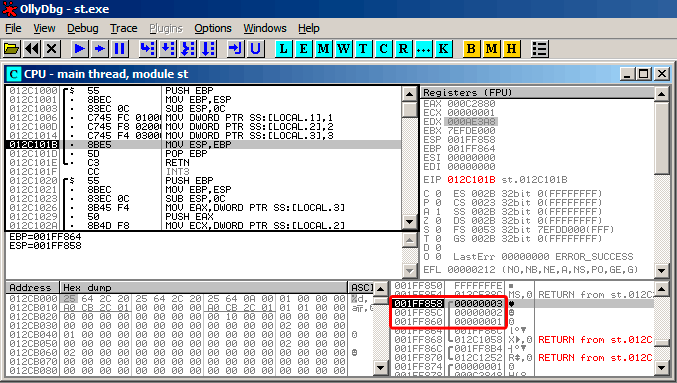
\includegraphics[scale=\FigScale]{patterns/02_stack/08_noise/olly1.png}
\caption{\olly: \TT{f1()}}
\label{fig:stack_noise_olly1}
\end{figure}

Когда \TT{f1()} заполняет переменные $a$, $b$ и $c$ они сохраняются по адресу \TT{0x1FF860} \etc{}.

\clearpage
А когда исполняется \TT{f2()}:

\begin{figure}[H]
\centering
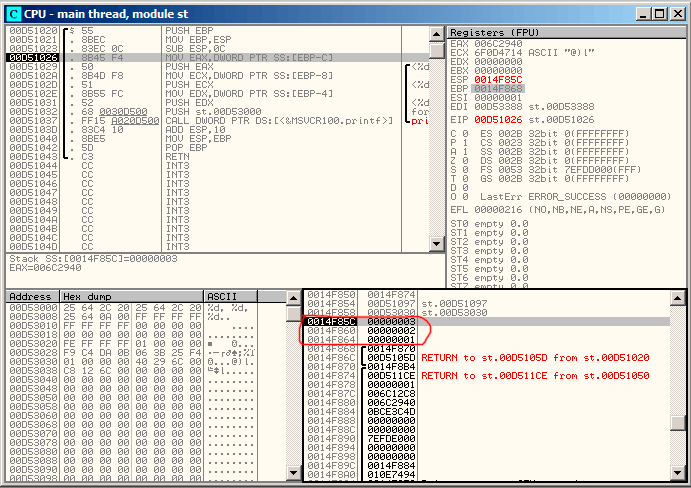
\includegraphics[scale=\FigScale]{patterns/02_stack/08_noise/olly2.png}
\caption{\olly: \TT{f2()}}
\label{fig:stack_noise_olly2}
\end{figure}

... $a$, $b$ и $c$ в функции \TT{f2()} находятся по тем же адресам!
Пока никто не перезаписал их, так что они здесь в нетронутом виде.
Для создания такой странной ситуации несколько функций должны исполняться друг за другом
и \ac{SP} должен быть одинаковым при входе в функции, т.е. у функций должно быть равное количество
аргументов). Тогда локальные переменные будут расположены в том же месте стека.
Подводя итоги, все значения в стеке (да и памяти вообще) это значения оставшиеся от 
исполнения предыдущих функций.
Строго говоря, они не случайны, они скорее непредсказуемы.
А как иначе?
Можно было бы очищать части стека перед исполнением каждой функции,
но это слишком много лишней (и ненужной) работы.

\subsectionold{MSVC 2013}

Этот пример был скомпилирован в MSVC 2010.
Но один читатель этой книги сделал попытку скомпилировать пример в MSVC 2013, запустил и увидел 3 числа в обратном порядке:

\begin{lstlisting}
c:\Polygon\c>st
3, 2, 1
\end{lstlisting}

Почему?
Я также попробовал скомпилировать этот пример в MSVC 2013 и увидел это:

\begin{lstlisting}[caption=MSVC 2013]
_a$ = -12						; size = 4
_b$ = -8						; size = 4
_c$ = -4						; size = 4
_f2	PROC

...

_f2	ENDP

_c$ = -12						; size = 4
_b$ = -8						; size = 4
_a$ = -4						; size = 4
_f1	PROC

...

_f1	ENDP
\end{lstlisting}

В отличии от MSVC 2010, MSVC 2013 разместил переменные a/b/c в функции \TT{f2()} в обратном порядке.
И это полностью корректно, потому что в стандартах \CCpp нет правила, в каком порядке локальные переменные должны быть размещены в локальном стеке, если вообще.
Разница есть из-за того что MSVC 2010 делает это одним способом, а в MSVC 2013, вероятно, что-то немного изменили во внутренностях компилятора, так что он ведет себя слегка иначе.

